\documentclass[tikz,border=5pt]{standalone}
\usepackage{times}
\usepackage{amsmath,amssymb}
\usetikzlibrary{positioning,fit,arrows.meta,backgrounds,shapes.geometric,calc,shadows,decorations.pathreplacing}

\begin{document}
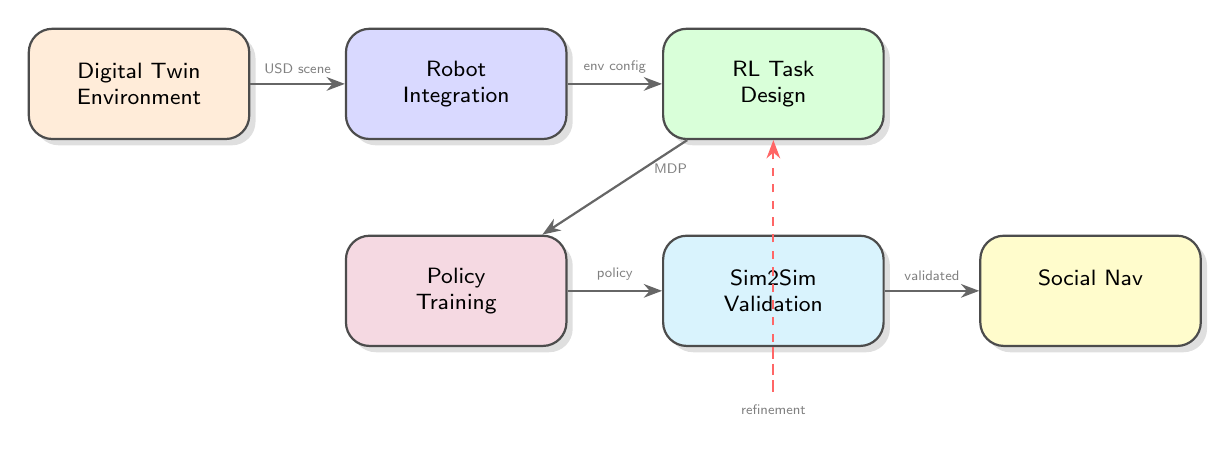
\begin{tikzpicture}[
    node distance=0.8cm and 1.5cm,
    phase/.style={
        draw=black!70,
        rounded corners=3mm,
        minimum width=2.8cm,
        minimum height=1.4cm,
        font=\sffamily\footnotesize,
        fill=white,
        thick,
        align=center,
        drop shadow={opacity=0.25, shadow xshift=0.08cm, shadow yshift=-0.08cm}
    },
    arrow/.style={->, >=Stealth, thick, color=black!60},
    label/.style={font=\sffamily\tiny, color=black!50}
]

\node[phase, fill=orange!15] (p1) {Digital Twin\\Environment};

% Phase 2
\node[phase, fill=blue!15, right=1.2cm of p1] (p2) {Robot\\Integration};

% Phase 3
\node[phase, fill=green!15, right=1.2cm of p2] (p3) {RL Task\\Design};

% Phase 4
\node[phase, fill=purple!15, below=1.2cm of p2] (p4) {Policy\\Training};

% Phase 5
\node[phase, fill=cyan!15, right=1.2cm of p4] (p5) {Sim2Sim\\Validation};

% Phase 6
\node[phase, fill=yellow!20, right=1.2cm of p5] (p6) {Social Nav\\};

% Arrows
\draw[arrow] (p1) -- node[above, label] {USD scene} (p2);
\draw[arrow] (p2) -- node[above, label] {env config} (p3);
\draw[arrow] (p3) -- node[right, label, pos=0.3] {MDP} (p4);
\draw[arrow] (p4) -- node[above, label] {policy} (p5);
\draw[arrow] (p5) -- node[above, label] {validated} (p6);

% Feedback loop
\draw[arrow, dashed, color=red!60] (p5.south) -- ++(0,-0.6) -| node[below, label, pos=0.25] {refinement} (p3.south);

\end{tikzpicture}
\end{document}
